\documentclass{article}

\usepackage[margin=1in]{geometry}
\usepackage{amsmath}
\usepackage{amssymb}
\usepackage{hyperref}
\usepackage{natbib}
\usepackage{setspace}
\usepackage{graphicx}

\begin{document}
\onehalfspacing % 1.5 line spacing

% Center the title section
\begin{center}
\rule{\linewidth}{1mm} \\[0.5cm]
{\Large\textbf{Evaluating the Impact of Weather on Capital Bikeshare DC Rides}}\\[0.3cm]
{\Large \textbf{Alexa Rossello}}\\[0.3cm]
{\Large \textbf{Fall 2024 Semester}}\\
\rule{\linewidth}{1mm} \\[0.2cm]
\end{center}

% Left-align the rest of the document
\section*{Problem Statement}
This project aims to understand how weather conditions affect bike share usage in Washington, DC for different types of riders. Specifically, the analysis investigates the relationship between weather factors and the daily count of bike rides. The goal is to understand how different weather conditions impact daily usage predictions for casual riders and members. Previous studies have shown that users respond differently to weather depending on their ridership type, with members being more resilient to poor weather compared to casual riders \cite{quach2020, kim2018}. For example, Quach and Malekian (2020) used k-means clustering to identify ridership patterns in Washington, DC, revealing that adverse weather decreases ridership among casual users, while members are less affected. Similarly, Kim (2018), focusing on South Korea, highlighted that temperature and precipitation considerably impact trip patterns, particularly for casual riders. This analysis contributes to the literature by building on Quach’s DC-based study with a predictive modeling approach, which quantifies specific relationships between weather variables and ridership patterns. Unlike Quach’s clustering modeling, this project employs Negative Binomial Regression and Random Forest models to predict ridership counts and interpret the effects of temperature, precipitation, and rider type. This regression-based approach complements Quach’s by offering actionable insights under varying weather conditions. 

\section*{Data Sources}
The analysis uses two datasets: Capital Bikeshare trip data spanning February to June 2023, and weather observations for Washington, DC, during the same period, both of which are sourced from Kaggle \cite{kaggle2023}. The trip data includes fields such as ride duration and user type (member or casual), which were used to calculate daily ride counts by rider type. The weather dataset contains information on daily average temperature, precipitation levels, and other meteorological variables. These datasets were merged on the date field to create a comprehensive dataset that links daily ride counts to corresponding weather conditions.


\section*{Methodology}
The data underwent several preprocessing steps to ensure it was suitable for analysis. Notably, weather conditions were categorized into temperature groups (\texttt{Cold}, \texttt{Moderate}, \texttt{Hot}) and rain groups (\texttt{No Rain}, \texttt{Light Rain}, \texttt{Heavy Rain}). Interaction terms between temperature and precipitation were introduced to capture how weather impacts differ for casual riders and members.

The Exploratory Data Analysis (EDA) focused on understanding the patterns in ridership and weather by visualizing daily ride counts, rider type distribution, and ride counts categorized by weather conditions.

\begin{figure}[h!]
\centering
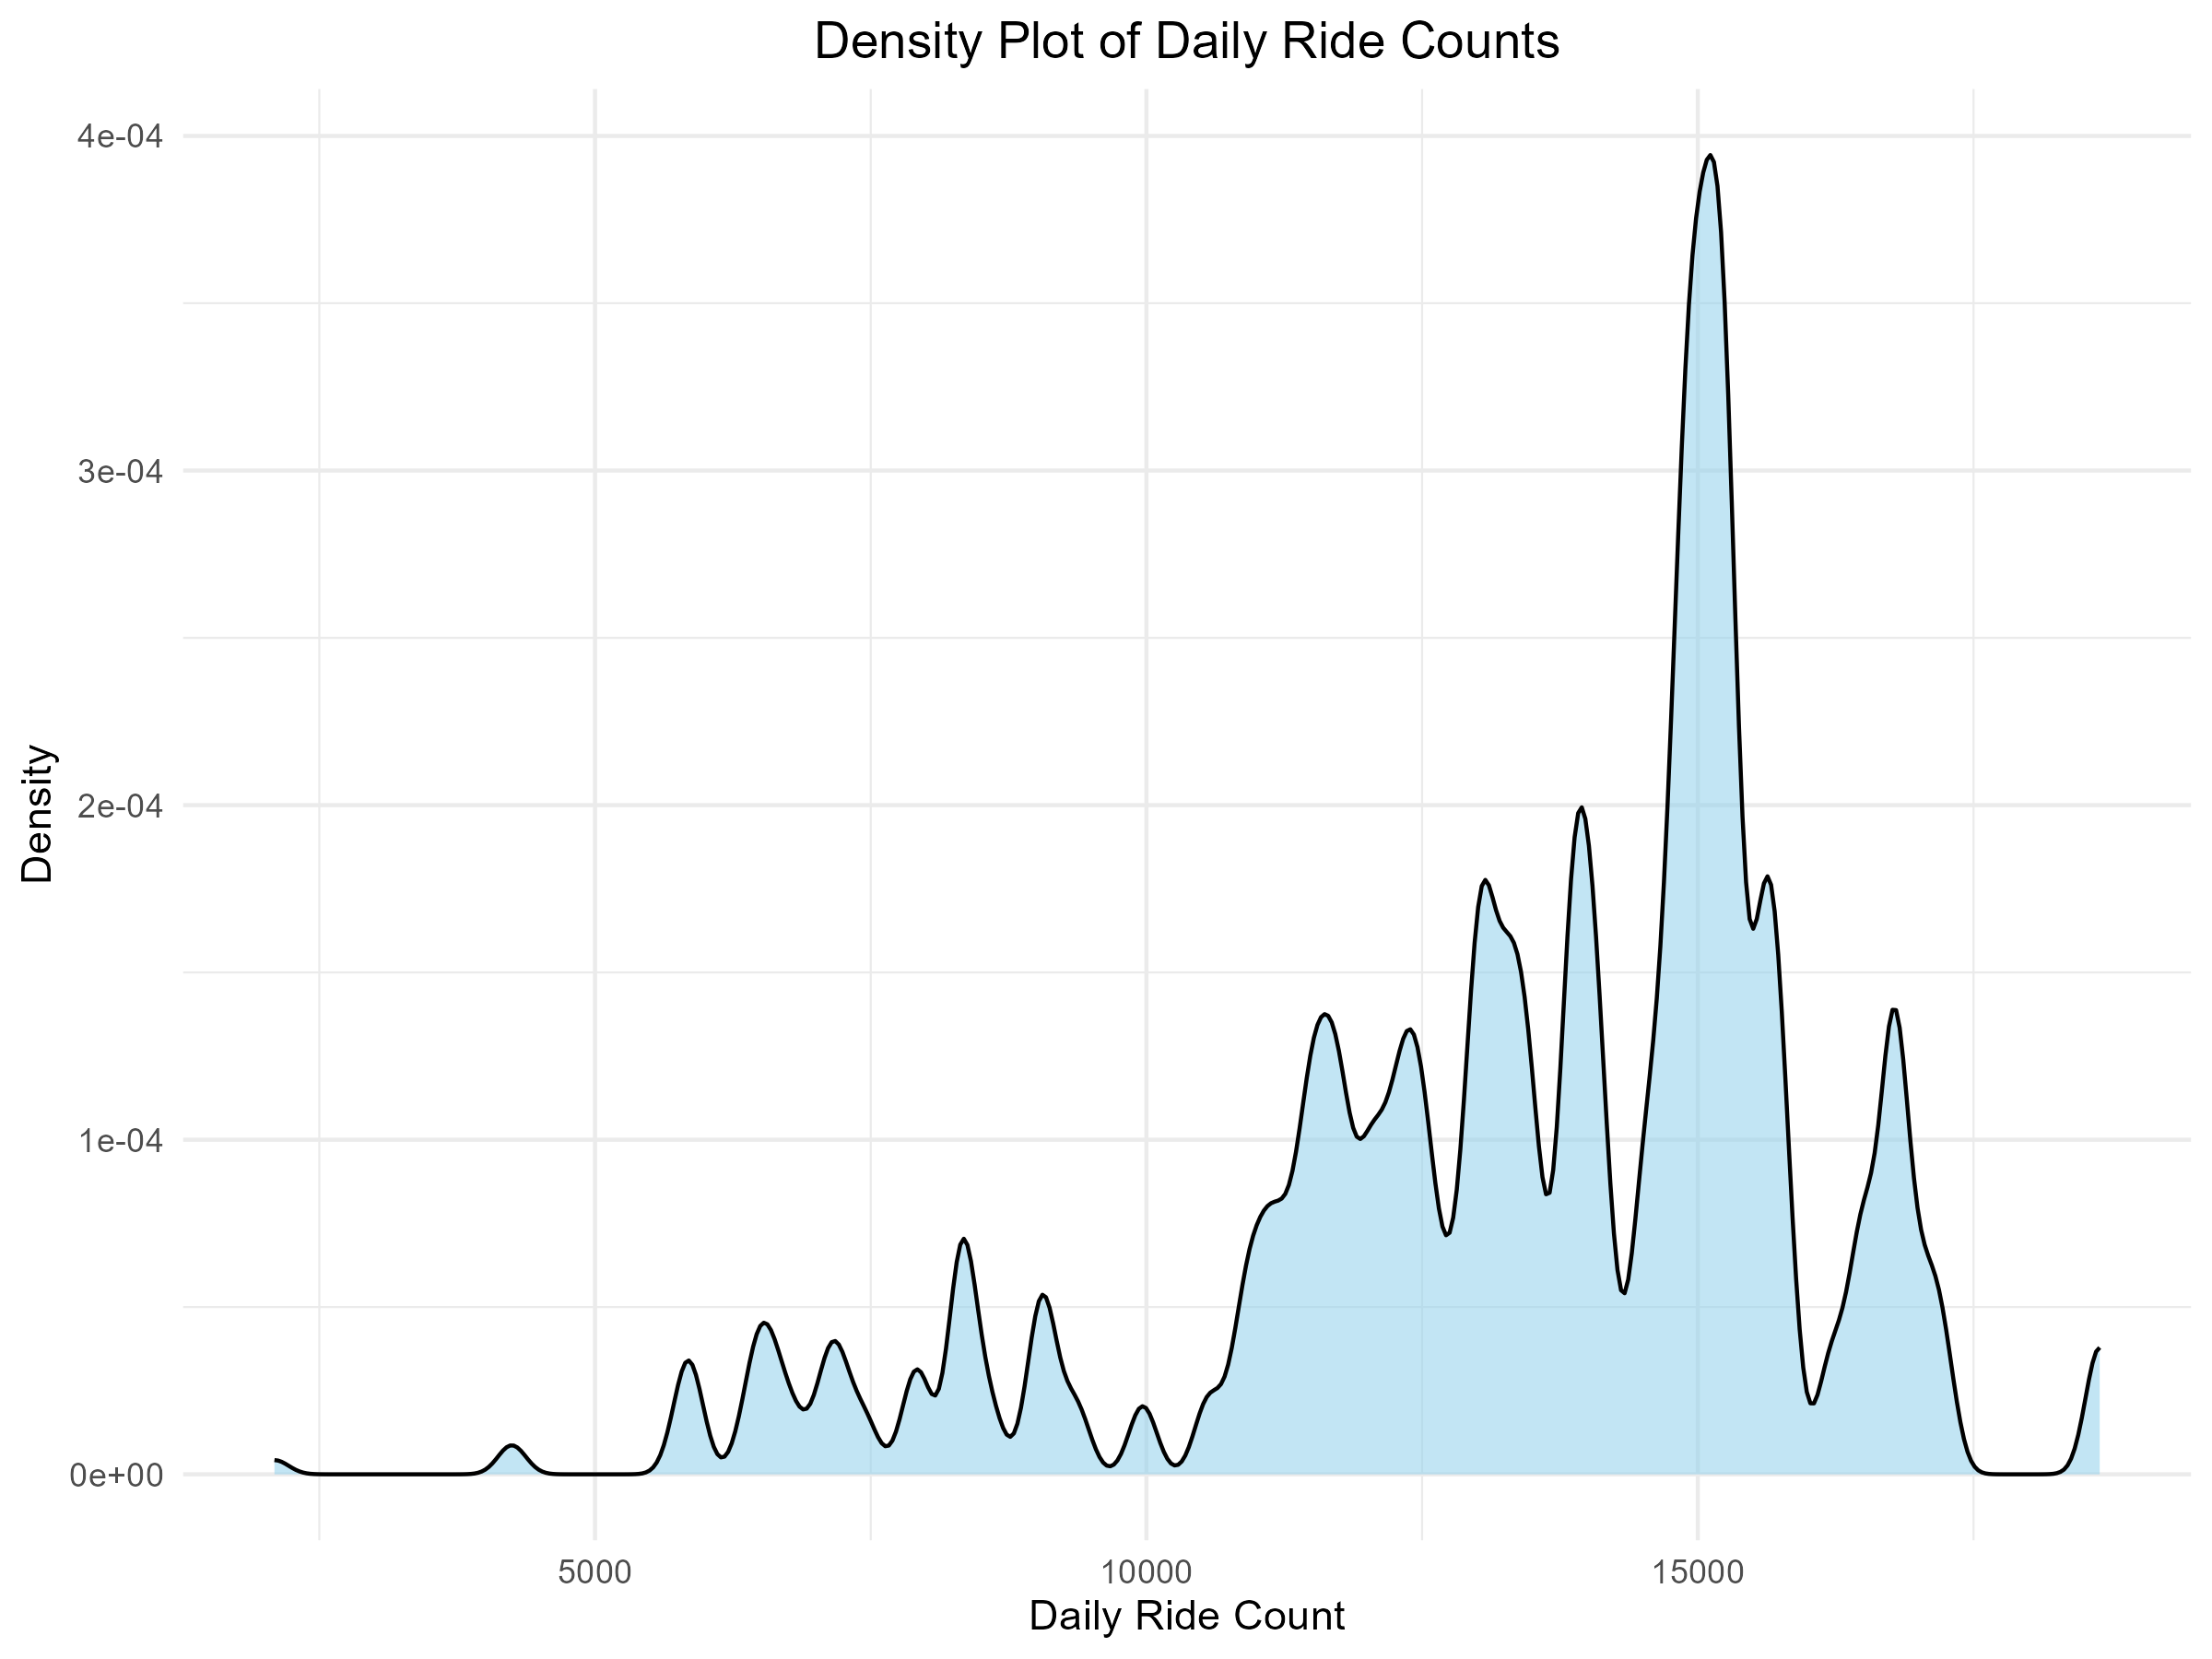
\includegraphics[width=0.7\textwidth]{daily_rides_density.png}
\caption{Density Plot of Daily Ride Counts}
\label{fig:ride_density}
\end{figure}

\begin{figure}[h!]
\centering
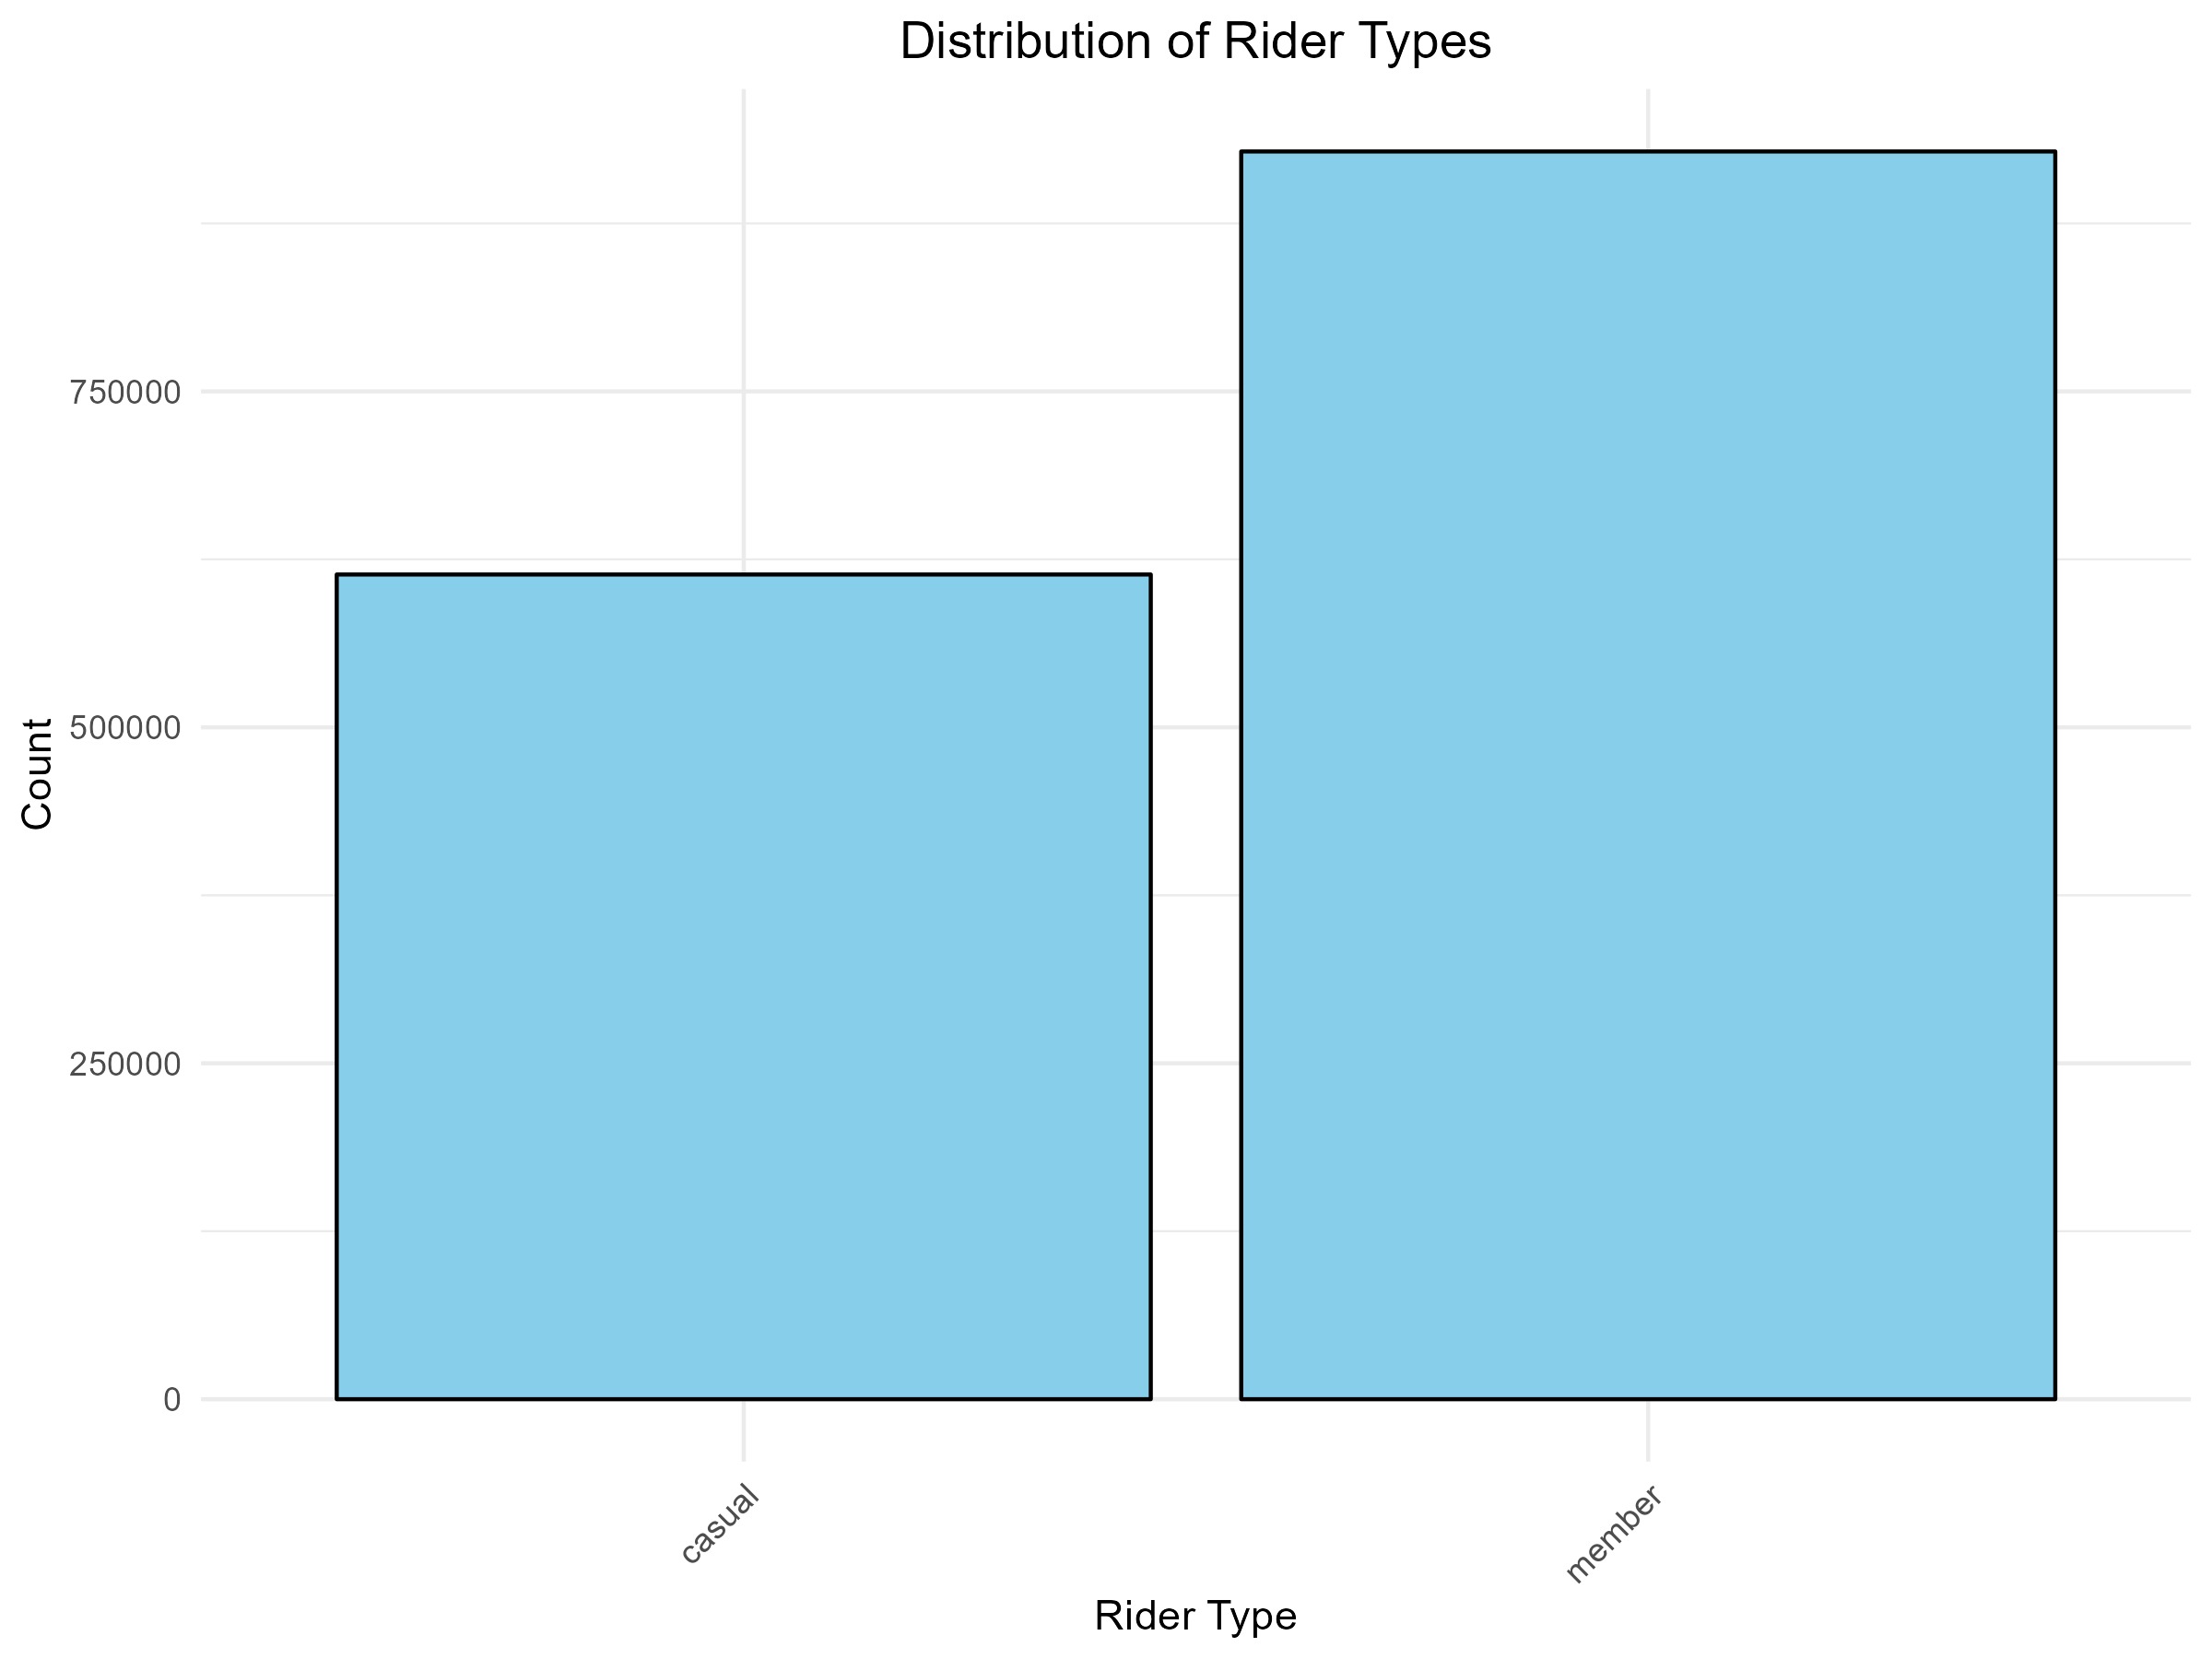
\includegraphics[width=0.7\textwidth]{rider_types.png}
\caption{Distribution of Rides by Rider Type}
\label{fig:rider_type_distribution}
\end{figure}

\begin{figure}[h!]
\centering
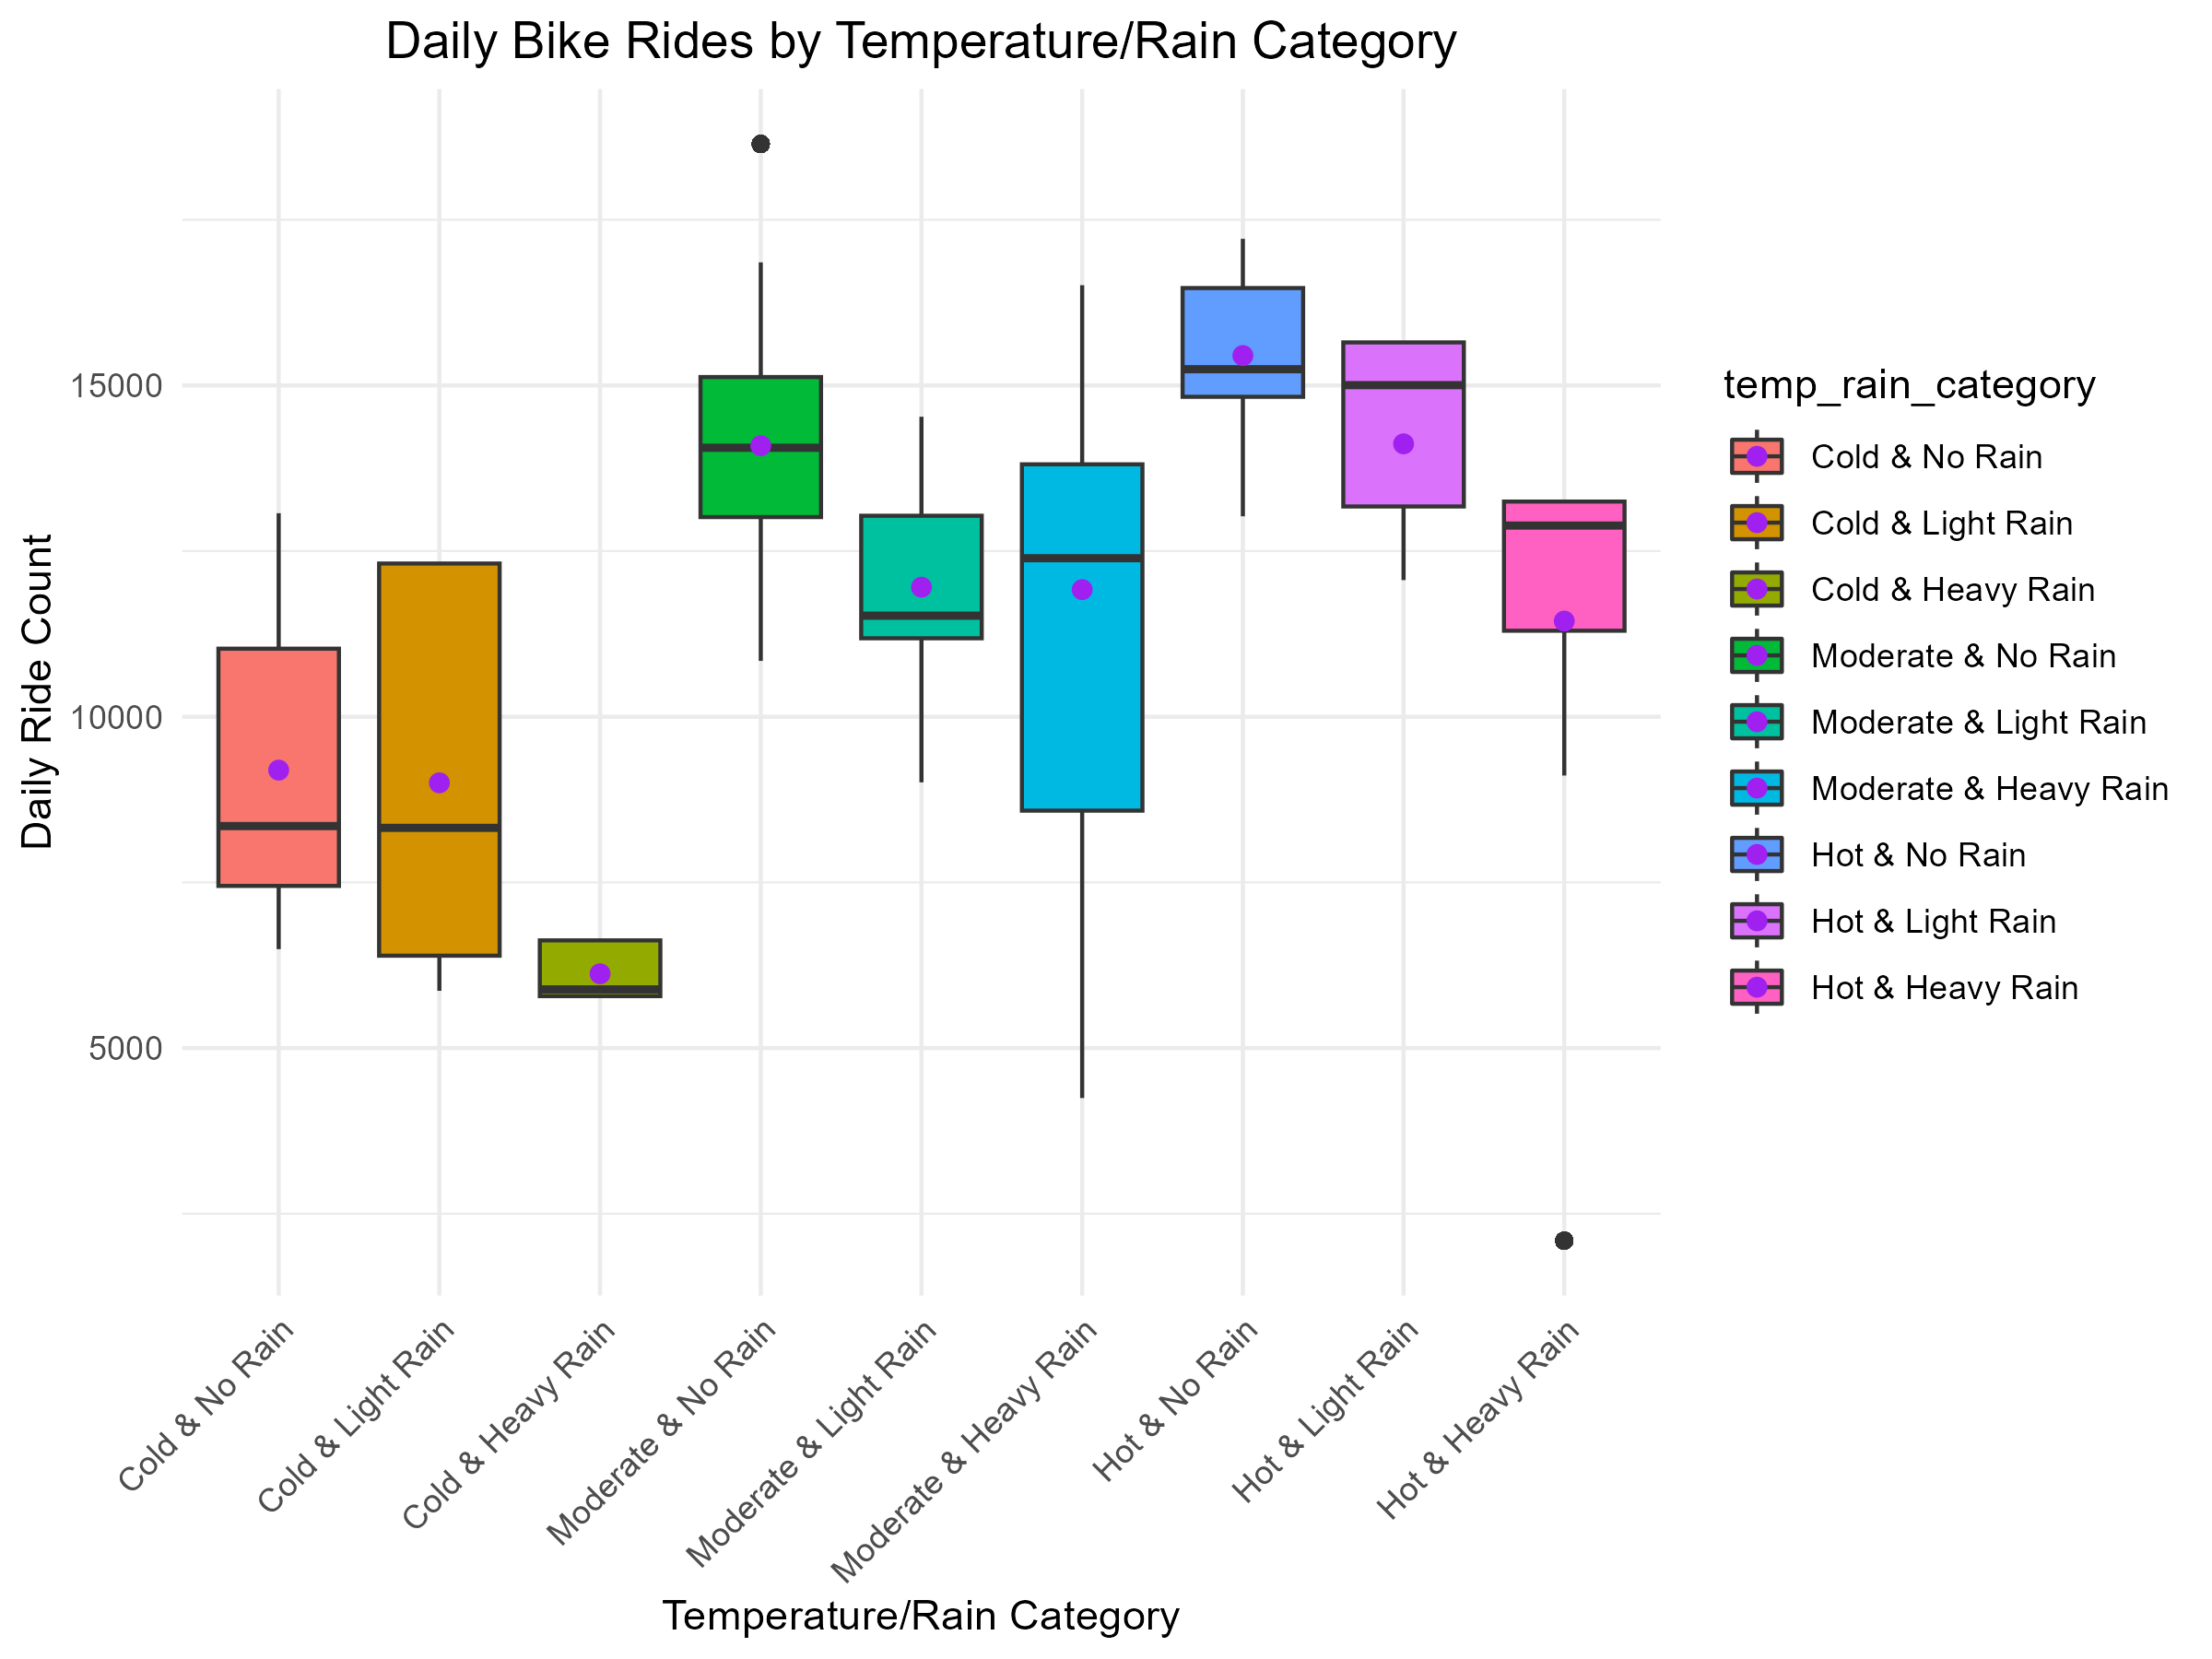
\includegraphics[width=0.8\textwidth]{boxplot_rides_temp.png}
\caption{Daily Ride Counts by Temperature and Rain Categories}
\label{fig:temp_rain_categories}
\end{figure}



Figure \ref{fig:ride_density} shows the density of daily ride counts, confirming a non-normal, multimodal distribution. This was confirmed by using the Shapiro-Wilk normality test. It found that the data grouped by weather conditions and user type significantly deviated from normality (\( p < 0.001 \)). The results of these tests led to the decision to use non-parametric statistical models. Figure \ref{fig:rider_type_distribution} illustrates the distribution of rides by rider type, showing that members account for the majority of rides. While, Figure \ref{fig:temp_rain_categories} displays daily rides segmented by temperature and rain categories. Ridership is highest under \texttt{Hot} temperatures with \texttt{No Rain}, while \texttt{Heavy Rain} leads to reduced rides regardless of temperature, particularly when there are extreme temperatures. 

To compare differences between \texttt{member} and \texttt{casual} riders under different weather conditions, the Mann-Whitney U test was applied. This test was used to evaluate differences in temperature and precipitation between the two groups. For temperature, the small p-value (\( p < 0.001 \)) indicates that there is a significant difference in the temperature distribution between member and casual riders. The test for precipitation yielded similar results, showing that two groups vary in their tolerance to precipitation. The examination of the medians for both weather types (temperature and precipitation) show that casual riders are more likely to be impacted by weather than members.

The Kruskal-Wallis test was used to examine the interaction between temperature and precipitation across weather categories (e.g., \texttt{Cold \& Heavy Rain} versus \texttt{Hot \& No Rain}). This test is a non-parametric alternative to one-way ANOVA and evaluates whether the distribution of daily ride counts differ significantly among multiple groups. Given the small p-value (\( p < 0.001 \)), post-hoc Dunn's tests were used to identify pairwise differences between weather categories. These tests revealed differences in ridership patterns across all weather categories, further confirming the impact of weather on bike share usage.

Following the EDA and subsequent statistical analysis, two predictive models were implemented: Negative Binomial Regression and Random Forest model. The Negative Binomial Regression model was chosen to address overdispersion in the data, where the variance exceeded the mean. The Random Forest model was used to evaluate the importance of predictors given its ability to handle non-linear relationships and interactions.

\section*{Evaluation and Final Results}
The Negative Binomial Regression model revealed several important relationships. In the context of negative binomial regression, the coefficients (\(\beta\)) are exponentiated (\(e^\beta\)) to interpret their effect on the expected count of daily rides. The intercept indicated a baseline log daily ride count of 8.57 when all predictors were zero. Temperature had a positive effect, with a 1°F increase leading to a 1.5\% increase in daily ride counts (\( \beta_1 = 1.0151, p < 0.001 \)). Precipitation had a substantial negative effect, with a 1-inch increase reducing daily ride counts by 47.5\% (\( \beta_2 = -0.6438, p < 0.001 \)). Interaction terms showed that casual riders were more sensitive to weather changes compared to members, further supporting the analysis completed thus far. Specifically, the positive interaction term for temperature and casual riders (\( \beta_3 = 0.002, p < 0.001 \)) indicates that temperature increases had a slightly stronger positive effect on casual riders than on members. Conversely, the negative interaction term for precipitation and casual riders (\( \beta_4 = -0.031, p < 0.001 \)) suggests that casual riders were more negatively impacted by rainfall. To generate predictions, a dataset was constructed using a grid of all combinations of predictor variables:
\begin{itemize}
\item \textbf{Temperature:} 100 evenly spaced values ranging from the minimum to the maximum observed temperatures.
\item \textbf{Precipitation:} Representative levels set to 0, 0.5, and 1.0 inches to capture scenarios such as no rain, light rain, and heavy rain.
\item \textbf{Rider Type:} Categorical variable with levels \texttt{casual} and \texttt{member}.
\end{itemize}

The predictions show how temperature, precipitation, and rider type interact to influence ridership patterns. Figure \ref{fig:temp_precip_ridership} illustrates the predicted daily ridership counts:

\begin{figure}[h!]
\centering
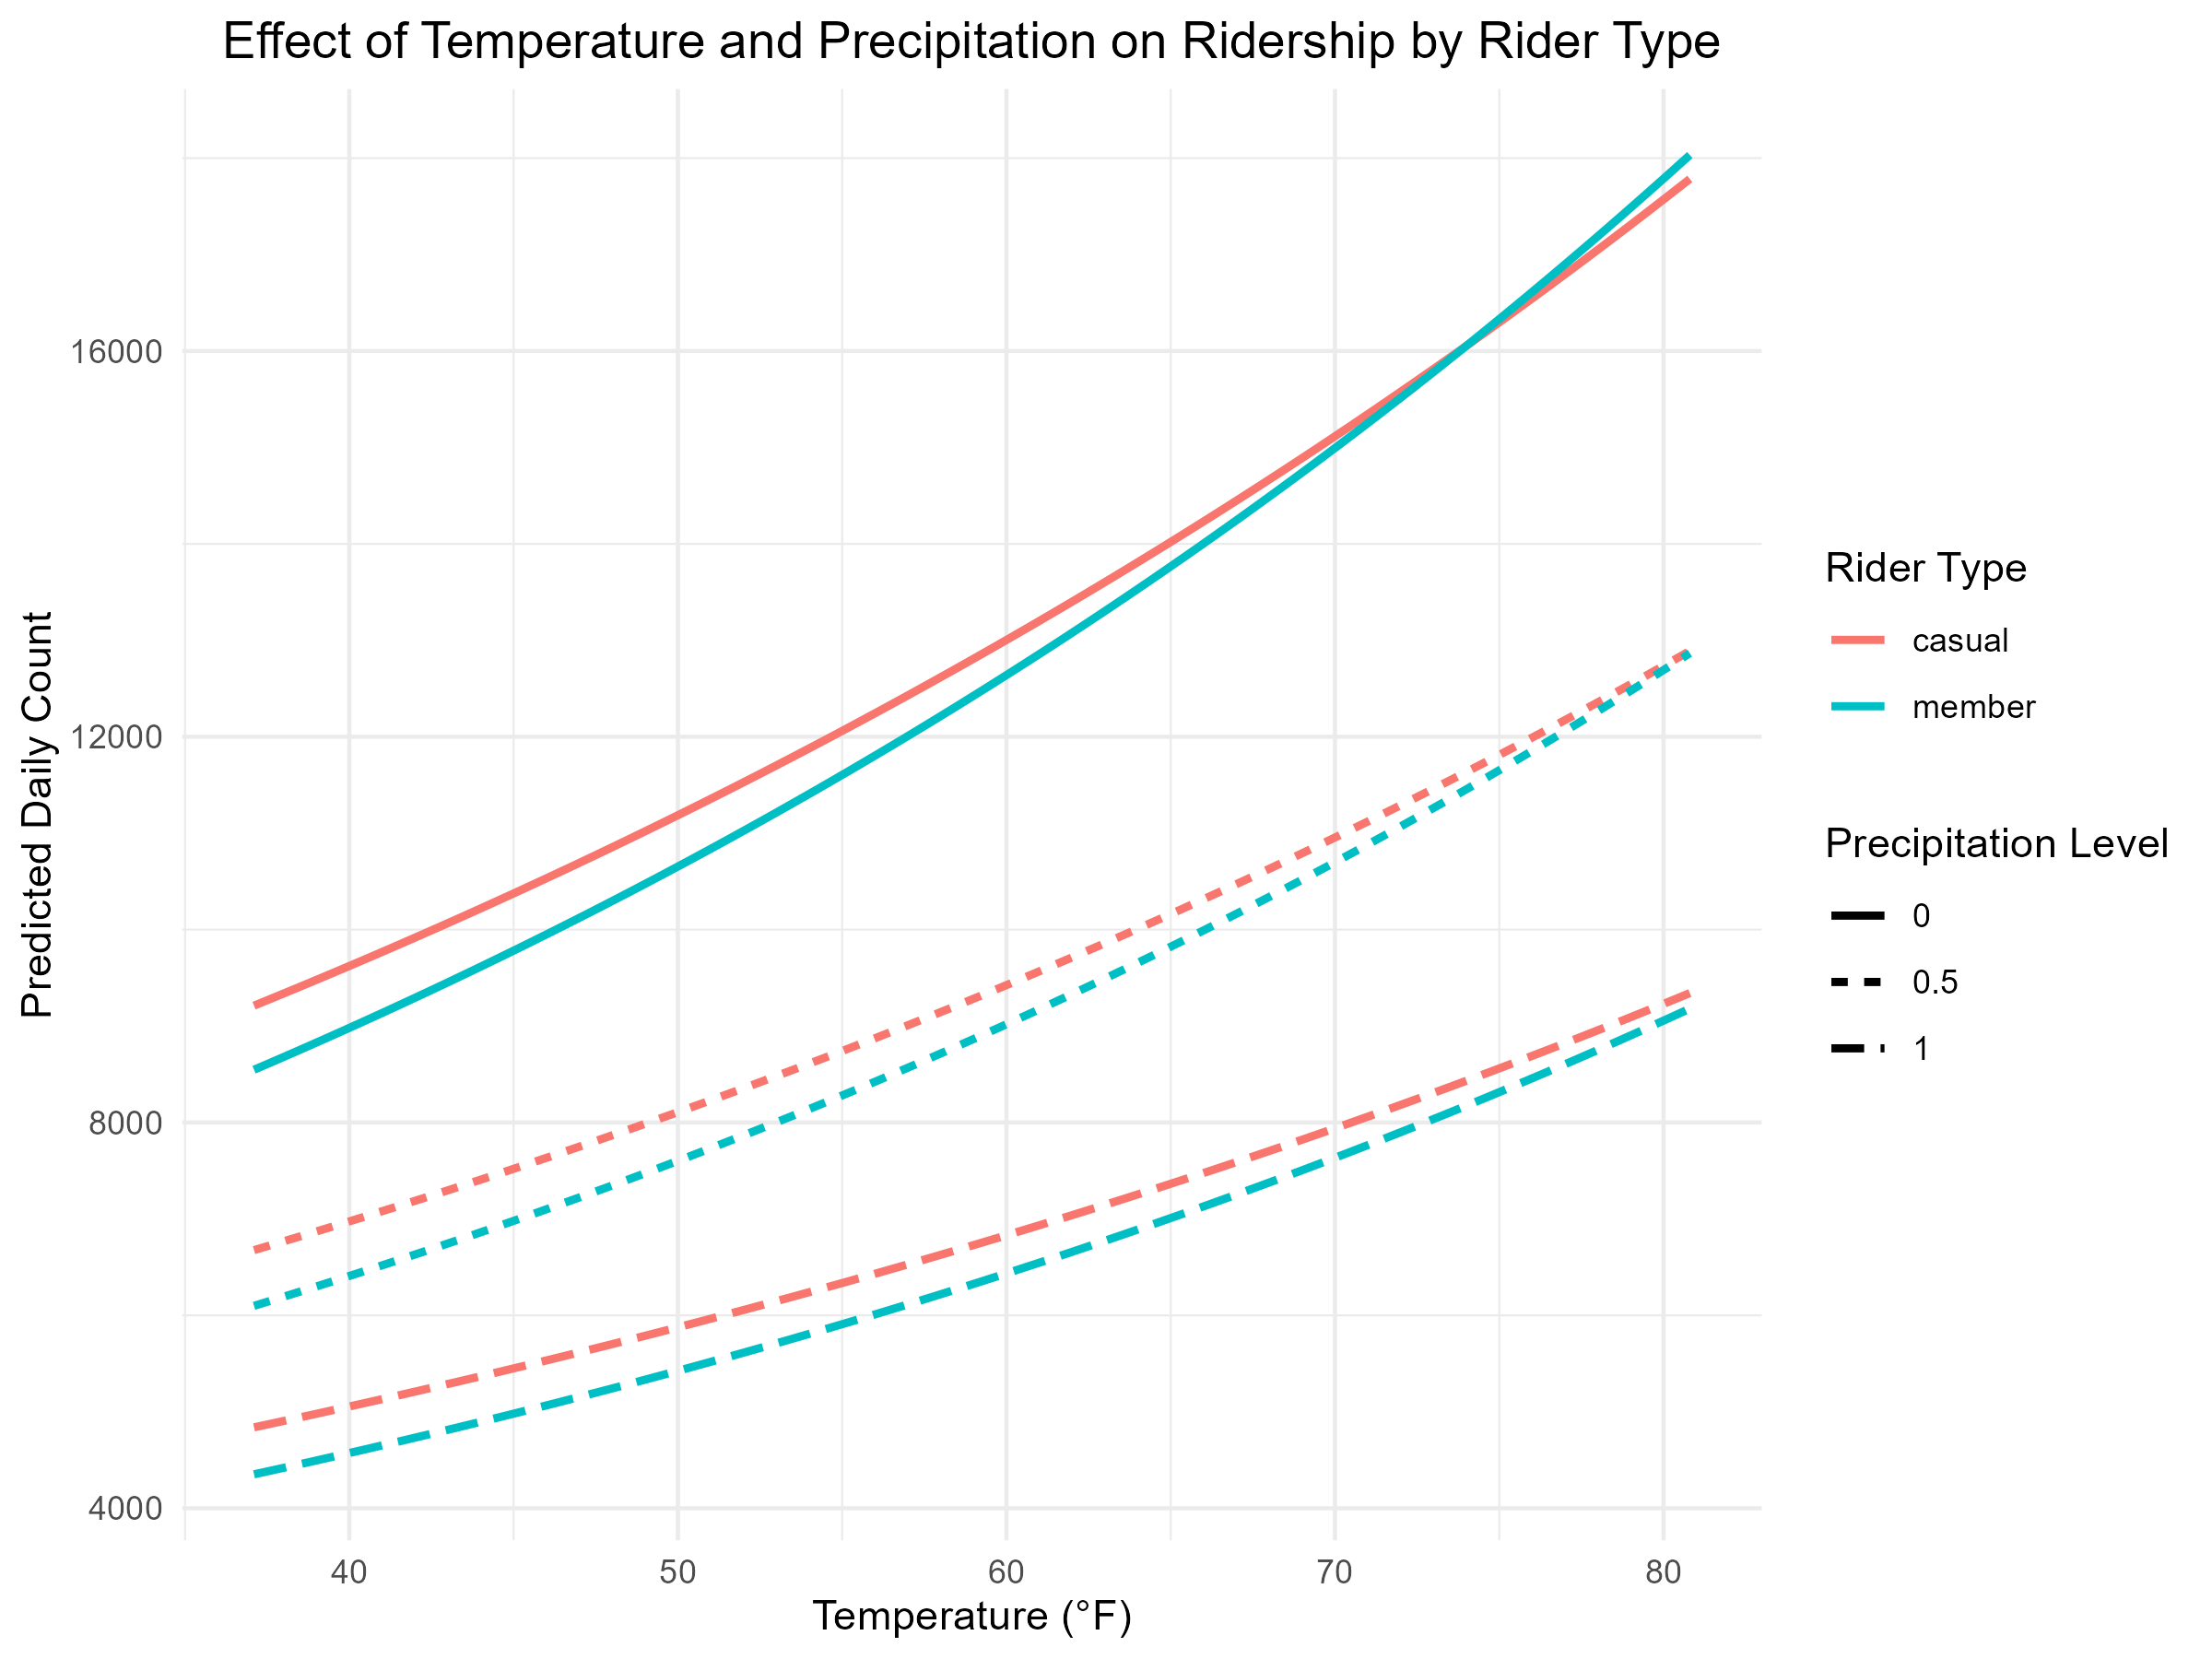
\includegraphics[width=0.8\textwidth]{reg_predictions.png}
\caption{Effect of Temperature and Precipitation on Ridership by Rider Type}
\label{fig:temp_precip_ridership}
\end{figure}


The Random Forest model explained 96.75\% of the variance in daily ride counts. As shown in Figure \ref{fig:rf_var_importance}, variable importance analysis ranked temperature as the most significant predictor, followed by precipitation and lastly membership status. This aligns with the findings from the regression model, where weather variables had the strongest influence on ridership patterns. The Random Forest model confirmed the non-linear relationship between weather and ridership, particularly in how extreme weather conditions amplify the sensitivity of casual riders compared to members. 

\begin{figure}[h!]
\centering
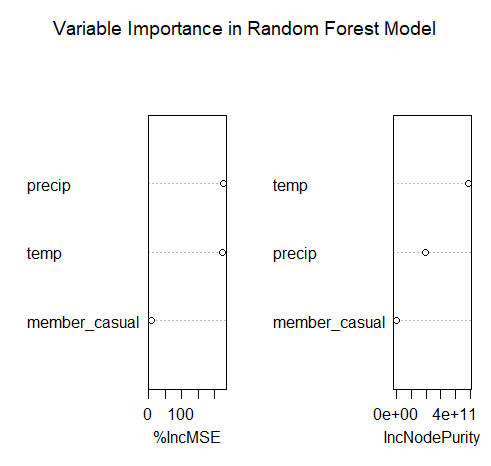
\includegraphics[width=0.6\textwidth]{varImpPlot.png}
\caption{Random Forest Model Variable Importance}
\label{fig:rf_var_importance}
\end{figure}

In conclusion, this study highlights the critical role of weather when predicting bike sharing usage. It is clear that casual riders are more affected by adverse conditions than members, and precipitation has a larger impact on ridership than temperature. While these results are not surprising, the analysis strongly supports the need to examine weather patterns to predict ridership and reinforces the analysis previously done by Quach and Malekian (2020). The results of this analysis can be used to incorporate the best practices from other urban areas with similar bike sharing programs, or introduce new innovations such as covered docking stations to improve the rider experience, especially for casual riders.

\newpage
\section*{Future Work} While this analysis provides valuable insights into the impact of weather on bike share usage, there are several opportunities for future research to expand upon these findings. First, incorporating a more robust dataset spanning multiple years would allow for the analysis of long-term trends and the inclusion of all four seasons, providing a more comprehensive understanding of seasonal variations. Additionally, future studies could explore differences in ridership patterns by day of the week or distinguish between workdays and weekends, which may reveal variations in commuting versus recreational usage.

Another potential area of exploration is incorporating geographic data to assess how weather impacts ridership across different regions of Washington, DC. Understanding spatial differences could help identify neighborhoods or routes that are more vulnerable to adverse weather conditions. Finally, integrating demographic data, such as rider age or income, could provide deeper insights into how weather impacts various user groups, informing more targeted operational strategies and marketing campaigns.

\newpage
\bibliographystyle{plainnat}
\bibliography{references}

\end{document}

